\chapter{研究背景}
本研究を理解する上で必要な概念である, 強化学習とそのアルゴリズムであるMA-POCAの理論や,関連する研究について述べる.
また,本研究を行うことになった社会的背景についても述べる.

\section{津波避難誘導における課題}
災害大国である我が国において,地震発生後の津波避難誘導オペレーションは非常に重要である.
特に近年,津波以外にも異常気象等による気象災害の激甚化もあり,避難誘導の遂行にあたって,益々その危険性も増していると推察される.\par 
本章では,我が国での津波避難誘導における課題について取り上げ,後述する提案手法の研究背景の理解を補助するものとする.
\subsection{オーバーツーリズムと観光地における避難誘導の課題}
近年の大幅な観光客増加と,観光地における避難誘導の課題,その関連性について述べる.
\paragraph{オーバーツーリズムとは}
\paragraph{観光地における避難誘導の課題}
\subsection{二次被害の発生}
津波避難誘導(あるいは,他の災害における避難誘導)においては,発災直後から二次被害にあう危険性が高い地域で活動しなければならないため,現場で誘導を行う警察や消防員等の安全確保が問題になっている.\par
\paragraph{風水害時における人的被害の特徴}
以下は,我が国で発生した1969年から2018年までの災害を対象に,消防団員が殉職した事例を消防白書や新聞記事,既往研究などから把握し,殉職時の状況を分析した結果が,山田らの研究\cite{yamada2020}によって報告されている.
\begin{quote}
  図-3 より,津波は,出動 途上,水防作業中,避難中,避難誘導中,人命救助中に 殉職者を出したことがわかった.なかでも避難誘導中と 避難中を合わせると全体で約 80\%を占めており,避難に関係する時に殉職者が出ている.
  \begin{figure}[H] 
    \centering 
    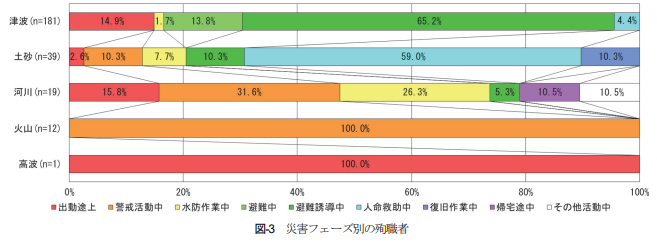
\includegraphics[width=0.8\textwidth]{Figures/fig-01.png}
    \caption{消防団員の災害フェーズ別殉職者の割合} 
    \label{fig:01} 
\end{figure}
\end{quote}
以上より,津波災害時の消防団員おけるの2次被害に関しては,避難誘導中が最も多い結果であることが示されている.上記は消防団員に限定した統計であるが,同じく避難誘導を行うすべての人員においても同様の傾向があると推察される.

  \subsection{災害時の必要人員不足}
\section{航空法改正によるドローンの災害対応における活用}
  \subsection{2022年12月5日の改正航空法の施行}
  \subsection{ドローンによる避難誘導の先行研究}
\section{強化学習}
%% TODO;機械学習と強化学習の基本的な枠組みについて述べる
  \subsection{MA-POCA(MultiAgent POsthumous Credit Assignment)}
  %% TODO: 協調学習:MA-POCAについての説明

